\section{提案システム}
本章では,DNSトンネリングの発生抑止を目的とした名前解決システムDNS-TD(DNS for Tunneling Deterrence)について説明する.
%第\ref{sec:related-works}で述べたように,これまでに提案されてきた検知に基づくDNS Tunneling対策には,Low Throughput手法および転送頻度を下げる手法に対して,検知が困難であるという課題がある.
%他方,新しいアーキテクチャに基づく名前解決システムには,マイグレーションの課題が残留している.
\begin{figure}[h]
 \centering
 \label{fig:abstruct-DNS-TD-architecture}
 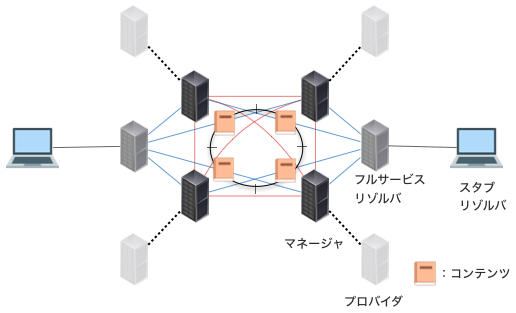
\includegraphics[scale=0.6]{figure/new-architecture-DNS-TD.png}
 \caption{提案システムの概略図}
\end{figure}

\subsection{概要}
\label{sec:DNS-TD}
%現在の課題
%目的をしっかりと説明すること
%現在使用されているDNSに基づく名前解決において,問い合わせのパケットを悪用することで任意のデータを送受信するキャリアとして悪用するDNSトンネリングという秘匿通信手法として利用される設計上の不備がある.
%検知に基づいた対策アプローチが過去に多数提案されているが,転送量および頻度を調整する迂回手法を用いる場合には対処するのに不十分であるという課題がある.
%DNSトンネリングは,クライアントからの名前解決クエリがコンテンツを保持するサーバに透過的に転送されることに起因して発生する.
%提案システムでは,この点に着目し,
%%そこで,DNSトンネリングが発生しない
%この課題に対して,トンネリング通信を抑止することを目的とする新しい名前解決システム(DNS-TD)を提案する.
%提案システムでは,クライアントからの名前解決問い合わせがコンテンツの操作と保持の機能を兼ねるサーバに転送されることに着目し,その機能を分離させることによって,トンネリング抑止を実現する.
%%フラットな名前空間と分散ハッシュテーブルの仕組みを利用することによるトンネリング通信の発生を抑止する名前解決システムを提案する.
%%設計要件
%提案システムのDNS-TDの主要な要素は,以下の通りである.
%\begin{itemize}
%% \item 84byteの名前空間における全てのコンテンツ情報をマップ
%% \vspace{-3mm}
% \item ゾーンをハッシュ空間の範囲に基づき分割
% \vspace{-3mm}
% \item 権威サーバにおけるレコード情報の操作機能と管理機能の分離
% \vspace{-3mm}
% \item ドメイン名ではなく識別子に基づく名前解決
% \vspace{-3mm}
% \item レコード情報に対する認証機能
%\end{itemize}
%ハッシュ値に基づくフラットな名前空間をソートした範囲に基づき分割し,コンテンツを保持する管理サーバによって分散的に管理する.
DNS-TDでは,クライアントからの名前解決クエリを処理するサーバは,コンテンツを操作する機能を持たないノードによって処理される設計になっている.
コンテンツ情報を変更する機能とクライアントにコンテンツを提供する機能を分離することによって,DNSトンネリングにおけるクライアントとコンテンツを操作するサーバとの通信の発生を抑止する.
また,DNS-TDでは,ゾーンファイルによって権威サーバによってドメインに紐付けるレコード情報を一元的に管理するのではなく,リソースレコードのタイプごとにコンテンツの識別子を付与し,識別子に基づき担当のサーバ,提案システムではマネージャによって分散的に管理される.
識別子は,224bitの名前空間をもつハッシュ関数によって算出されるメッセージダイジェストを利用する.
レコード情報を操作するのは,実際にレコード情報を保持するマネージャではなく,マネージャに階層的に連結したプロバイダと呼ばれるサービスノードである.
マネージャは,プロバイダからのレコード情報に対する操作リクエストに基づいて,担当のマネージャに転送する.
DNS-TDの名前空間は,ソートされたハッシュ値の範囲に基づき分割され,既存システムのTLDによって分割された範囲をゾーンとして分割的に管理される.
DNS-TDにおけるクライアントは,シンボルを算出することによって,レコード情報を保持するノードを一意に特定することができる.
また,シンボルからレコード情報を保持するノードを一意に特定の名前解決プロセスでは,レコード情報を作成したエンティティは介在されない.
すなわち,レコード情報を作成する機能とレコード情報を管理する機能を異なるサービスノードに分離させることによって,DNS-TDではDNS Exfiltrationが発生することを抑止する.

DNS-TDでは,DNS Infiltrationに対して,認証基盤の導入と使用できるリソースレコードを制限するメソッドを採用する.
認証基盤では,ドメインに関連づけるレコード情報との関連性を評価することで不審なレコード情報がハッシュテーブル上にストアされることを防止する.
Qnameにシンボルとして224bitのメッセージダイジェストを使用することによって,副次的効果として,偽装DNS応答パケットの作成が困難にできるという性質が期待される.
また,既存システムにおけるDNSSECによって実現されてきた送信元のトレーサビリティについて,DNS-TDでは認証基盤とシンボルに基づくDNS応答パケットの偽装困難性によって実現され,DNSSECの必要性はなくなる.
さらに,任意の文字列を注入することができるレコードタイプ``NULL"と``TXT"について,実験目的のNULLタイプの使用制限とTXTタイプは機能をシンタックスの限定しているSPFに回帰させることで対処する.
DNS-TDにおける用語については,表~\ref{tab:refres-terminology}で示す.
\begin{table}[h]
 \centering
  \begin{tabular}{cl}
    \toprule
    \multicolumn{1}{c}{\textbf{表記}} & \multicolumn{1}{c}{\textbf{意味もしくは機能}}\\
    \midrule

    コンテンツ & \begin{tabular}{l}・識別子に関連づけられたレコード情報の実体\end{tabular}\\ \hline

    コンテンツID & \begin{tabular}{l}・識別子\end{tabular}\\ \hline

    レコード情報 &
      \begin{tabular}{l}
        ・リソースレコードの具体的な値\\
        (E.g. IPアドレス)
      \end{tabular}\\ \hline

     リソースレコードタイプ &
      \begin{tabular}{l}
        ・オブジェクトに関連づけるリソースレコードの型\\
        (E.g. A, AAAA, MX)
      \end{tabular}\\ \hline

    オブジェクト &
      \begin{tabular}{l}
       ・問い合わせる対象\\
       (E.g. ドメイン名もしくはIPアドレス)
      \end{tabular}\\ \hline

    スタブリゾル & \begin{tabular}{l}・名前解決クライアント\end{tabular}\\ \hline

    フルサービスリゾルバ &
      \begin{tabular}{l}
       ・スタブリゾルバからのクエリハンドリング\\
       ・識別子の作成
      \end{tabular}\\ \hline

    マネージャ &
      \begin{tabular}{l}
       ・フルサービスリゾルバからのクエリハンドリング\\
       ・ゾーンの管理\\
       ・コンテンツの保持
      \end{tabular}\\ \hline

    プロバイダ & \begin{tabular}{l}・コンテンツの作成・更新・削除操作\end{tabular}\\

    \bottomrule
  \end{tabular}
 \label{tab:refres-terminology}
 \caption{SORESにおける用語}
\end{table}


\newpage
\subsection{システムアーキテクチャ}
\begin{figure}[htbp]
 \centering
 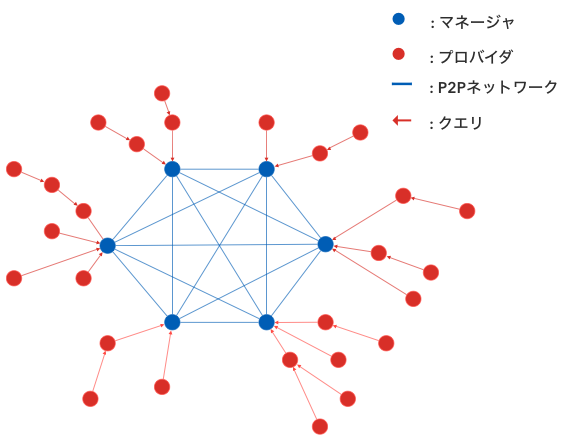
\includegraphics[scale=0.5]{figure/manager-provider.png}
 \caption{マネージャとプロバイダの関係図}
 \label{fig:manager-provider}
\end{figure}

DNS-TDでは,全体のアーキテクチャを従来のクライアントサーバアーキテクチャを踏襲している.
クライアントサーバアーキテクチャを採用することによって,クライアントは既存のDNSサービスに変更を加えることなく使用することができる.
他方で,サーバ同士はフルメッシュなネットワークで構成される.
%なぜこのアーキテクチャにしたのか

\subsection{サービスノード}
DNS-TDを構成するサービスノードは,以下の4つである.
\begin{itemize}
 \item スタブリゾルバ
	\vspace{-3mm}
 \item フルサービスリゾルバ
	\vspace{-3mm}
 \item マネージャ
	\vspace{-3mm}
 \item プロバイダ
\end{itemize}

DNS-TDでは,権威サーバが機能に基づき二つサービスノードに分割される.
DNS-TDでは,既存のDNSにおける権威サーバの機能を二つのサービスノードで動作させることによって,DNSトンネリングの抑止を図る設計になっている.
権威サーバの機能を列挙すると以下のようになる.
\begin{itemize}
 \item 上位ドメインから委任されたゾーンを管理する機能
	\vspace{-3mm}
 \item レコード情報を保持する機能
	\vspace{-3mm}
 \item スタブリゾルバからの名前解決問い合わせに応答する機能
	\vspace{-3mm}
 \item レコード情報を作成・修正・削除する機能
\end{itemize}
DNSトンネリングは,これら機能と性質を組み合わせることで発生する手法である.
例えば,スタブリゾルバから権威サーバ方向のデータ転送手法であるDNS Exfiltrationは,``スタブリゾルバからの名前解決問い合わせに応答する機能"と``"を組み合わせることで機能する.
また,権威サーバからスタブリゾルバ方向のデータ転送手法であるDNS Infiltrationは,``スタブリゾルバからの名前解決問い合わせに応答する機能"と``ゾーン内のレコード情報を作成・修正・削除する機能"が組み合わさることで機能するとそれぞれ捉えられる.
そこで,DNS-TDでは,権威サーバの機能を二つのサービスノード(マネージャとプロバイダ)に分けることで,既存の名前解決機能とDNSトンネリング抑止機能を実現する.\newline

\hspace{-12pt}\textbf{スタブリゾルバ}\\
\hspace{12pt}スタブリゾルバは,既存のDNSと同様,ドメイン名に関連づけられたリソースレコード情報を問い合わせるクライアントである.
DNS-TDが,既存のシステムと大きく異なるのは,問い合わせられたドメイン名とそのレコードタイプからコンテンツIDを識別子とすることで,レコード情報を解決する点である.
これを実現するために,既存システムのフルサービスリゾルバと権威サーバに変更が加えられ,機能が分割している.\newline

\hspace{-12pt}\textbf{フルサービスリゾルバ}\\
\hspace{12pt}フルサービスリゾルバは,従来システムと同様のキャッシュ機能を担いながら,コンテンツIDの算出し,コンテンツを保持するマネージャに問い合わせるサービスノードとして機能する.
フルサービスリゾルバは,スタブリゾルバからの従来のフォーマットのDNSクエリについて,ドメイン名とレコードタイプからハッシュ値の算出を行う機能を担う.
\begin{algorithm}[htbp]
 \caption{フルサービスリゾルバにおける問い合わせ転送処理}
 \label{algo:full-service}
  \SetKwProg{Fn}{}{\string:}{}
  \SetKwFunction{Handle}{handler}
 $\vspace{-0.3cm}$\;
% クエリハンドリング\;
 \Fn{\Handle{query\_data,\ rtype}}{
   $content\_id,\ domain\_id \leftarrow calculate\_id(query\_data,\ rtype)$\;
	 $manager\_addr \leftarrow find\_manager(start,\ end,\ content\_id)$\;
	 $answer \leftarrow query\_manager(manager\_addr,\ content\_id,\ domain\_id)$\;
	 $response\_client(client\_address,\ qname,\ answer.rcode,\ answer.rdata)$\;
 }
 $\vspace{-0.3cm}$\;
\end{algorithm}


\newpage
\hspace{-12pt}\textbf{マネージャ}\\
\hspace{12pt} マネージャは,ドメイン名に対応するレコード情報を保持し,フルサービスリゾルバからの問い合わせに応答するサービスノードである.
マネージャは,既存のDNSにおけるTLDに相当する権威サーバが担当する.
%マネージャの数
%イベントドリブン
%非同期
%フルサービスリゾルバからのクエリがあった時の動作を参考として説明する
\begin{algorithm}[htbp]
 \caption{マネージャにおける名前解決問い合わせ処理}
 \label{algo:query-process}
  \SetKwProg{Fn}{}{\string:}{}
  \SetKwFunction{Handler}{handler}
  \SetKwFunction{Parse}{parser}
  \SetKwFunction{Database}{db\_accesser}
  \SetKwFunction{Noerror}{generate\_packet}
  \SetKwFunction{Error}{generate\_errror}
 $\vspace{-0.3cm}$\;
 %Calculate the content'{}s content id and domain id\;
 \Fn{\Handler{query\_data}}{
	 $content\_id,\ qtype \leftarrow parser(query\_data)$\;
	 $record\_value \leftarrow db\_accesser(content\_id)$\;
	 \If{$value$}{
		 $payload \leftarrow benigh\_response(content\_id,\ qtype,\ ttl,\ record\_value) $\;
		}
		\Else{
		 $payload \leftarrow error\_response(content\_id,\ qtype)$\;
		 }
		$payload \leftarrow payload.pack()$\;
		$sendto(payload,\ client\_address)$\;
 }

%クエリのパース\;
% %Calculate the content'{}s content id and domain id\;
% \Fn{\Parse{data}}{
%   $payload = DNSRecord.parse(data)$\;
%	 $return \ {'packet\_id':payload[0], 'content\_id':payload[1], 'q\_type':payload[2]}$\;
% }
%
%
% $\vspace{-0.3cm}$\;
% %Find the manager who has zone includes the content id\;
% DBへアクセス\;
% \Fn{\Database{content\_id}}{
%	$return \ Redis("127.0.0.1", 6379).get(content\_id)$\;
% }
% $\vspace{-0.3cm}$\;
%
% %Query the content to the manager\;
% 応答パケットの作成\;
% \Fn{\Noerror{packet\_id, content\_id, q\_type, ttl, record}}{
%	$payload = DNSRecord(DNSHeader($\;
%				$qr=1, aa=1, ra=1,id=packet\_id, rcode=RCODE["NoError"]))$\;
%	$payload.add\_question(content\_id, q\_type)$\;
%	$payload.add\_answer(c\_id, ttl, record)$\;
%  $return \ payload$\;
% }
% $\vspace{-0.3cm}$\;
%
% %Transfer the answer to client\;
% エラー応答パケットの作成\;
% \Fn{\Error{packet\_id, content\_id, q\_type, ttl, record}}{
%	$payload = DNSRecord(DNSHeader($\;
%				 $qr=1, aa=1, ra=1,id=packet\_id, rcode=RCODE["NXDomain"]))$\;
%	$payload.add\_question(content\_id, q\_type)$\;
%  $return \ payload$\;
% }
\end{algorithm}


\hspace{-12pt}\textbf{プロバイダ}\\
%マネージャとのどのような階層構造なのか
%どのようなプロトコルでパケットをマネージャに転送するのか
\hspace{12pt}プロバイダは,レコード情報を作成・更新および消去といった操作を担当するサービスノードである.
プロバイダは,既存のDNSにおけるSLD以降の権威サーバに相当し,ドメインの階層構造を従いマネージャに接続される.
プロバイダは,マネージャを介在することで,レコード情報を操作することができる.
例えば,example.comプロバイダが``www"のIPアドレス情報を作成することを考える.
example.comプロバイダは,``www.example.com"とレコードタイプ``A"およびその値``93.184.216.34"を含むデータを接続先のcomマネージャにリクエストする.
comマネージャは,リクエストされたドメイン名とそれに関連づけるレコードタイプから識別子を算出し,担当のマネージャにストアリクエストを転送するという具合で動作する.

\newpage
\subsection{名前空間}
本項では,レコード情報にアクセスするために用いる識別子,コンテンツIDとその名前空間について説明する.
既存のDNSの名前解決システムでは,正引きをする際,ドメイン名とレコードタイプの二つの情報をキーとして,サーバは保持するゾーンファイルから該当するレコード情報が求まる.
他方,DNS-TDでは,ドメイン名とレコードタイプに基づき算出されるコンテンツIDを識別子として指定することでレコード情報にアクセスする.

におけるレコード情報へのアクセス方法は,識別子をキーとすることでデータを取得することができる.
コンテンツIDと呼ぶ,この識別子は,ドメイン名とレコードタイプの順番でその文字列の和を引数とするメッセージダイジェストで表現することができる.
例えば,ドメイン名を``www.example.com",レコードタイプを``A"とした場合,引数となるのは``www.example.comA"という具合である.
%以上のことから,224bitの名前空間をDNS-TDでは採用する.
% 224bitの名前空間を持つこととダイジェストの長さは違う
% sha3_224のダイジェスト長は,56文字

\subsubsection{ハッシュアルゴリズム}
続いて,DNS-TDが採用するハッシュアルゴリズムについて説明する.
DNS-TDでは,全てのコンテンツIDがフラットな名前空間上にマップされる.
従来では,異なるリソースレコードタイプのレコード情報について一つのゾーンファイルに記述することで,管理することができた.
他方で,DNS-TDでは,ドメイン名とリソースレコードタイプの組をハッシュ値の引数とするため,コンテンツIDは,レコード情報の数に比例して増加する特性がある.
また,識別子の引数の一つにドメイン名が含まれていることから,識別子から元のメッセージが導き出くことが困難な性質を備えていなくてはならない.
この性質を満たすことで,なんらかの方法で識別子を悪意の第三者が取得した際にDNS Exfiltrationとして機能してしまうことを抑止することができる.
最後に,DNS-TDでは,既存のDNSのプロトコルフォーマットを流用する設計になっているため,識別子が格納されるDNSのQuestion SectionのQnameのサイズ制約を満たさなくてはならない.
Qnameは,ラベルの最大長が63byteとする任意長の領域である.
以上のことを踏まえて,本システムにおけるハッシュアルゴリズムの要件は,以下の通りである.

\begin{enumerate}
 \item 名前空間は不足を無視できる程度に大きくなくてはならない
 \vspace{-3mm}
 \item アルゴリズムは一方向性の性質を備えなくてはならない
 \vspace{-3mm}
 \item ラベル長は最大63byte,ドメイン長は最大253byteである
 \vspace{-3mm}
\end{enumerate}

%ここで,既存のハッシュ関数の特性をまとめたtableを示す.

上記の内容から,DNS-TDでは,56byteの名前空間をもつsha3のアルゴリズムを採用する.

続いて,分離連鎖法と2重ハッシュ法によるコリジョン対策方法について説明する.
DNS-TDでは,コンテンツのストアリングフェーズでIDにコリジョンが発生した場合,分離連鎖法に基づきストアされるハッシュテーブルに連結リストという形式でコンテンツがストアされる.
リスト構造で延長するコンテンツの識別には,ドメインIDを識別子として利用する.
ドメインIDは,コンテンツIDと同様のハッシュアルゴリズムを用いて算出されるメッセージダイジェストの先頭32bitで表現される,ドメイン名を引数として生成される識別子である.
例えば,ドメイン名を``www.example.com"とする場合,そのメッセージダイジェストが``86ff20100c058b857bae9785bf0267e6c6afb740c18b8e9a87258485"であるとすると,``86ff"がドメインIDとなる具合である.
このように算出されたドメインIDは,DNSのQuestion Sectionのうち,それぞれ16bit分の領域を持つタイプとクラスの領域に埋め込まれる.
上記の仕組みによって,コリジョンが発生した際には,ドメインIDをキーとしてコンテンツを識別する.


\subsubsection{ゾーン分割}
本項では,ゾーンの分割方法およびマネージャノードのアドレスとそのゾーンの範囲に関する対応表について説明する.
はじめに比較のために,従来のシステムの場合について説明する.
従来のシステムでは,ドメインの階層構造に従い,ドメインの管理ノードを下位のドメイン管理ノードに委譲することでゾーンが分割される.
この仕組みでは,ゾーン内の全てのレコード情報はゾーンファイルに画一的にまとめられ,そのゾーンを管理する権威サーバがレコード情報の保持機能とクライアントから応答するという二つの機能を担う.
このゾーン分割メソッドでは,レコード情報の帰属が明確であり,ドメインの管理ノードがトラストアンカーとしての役割を同時に担うことができるメリットがある.
一方のDNS-TDでは,識別子を算出する際に使用するハッシュ関数によって構成される名前空間に基づき,ソートされたハッシュの名前空間の連続した範囲で分割する.
この分割された連続した範囲に基づきゾーンがマネージャに割り当てられることで,既存システム同様にレコード情報全体を分散的に管理する.

上記で説明するように,マネージャが管理するゾーンは,ハッシュの名前空間の連続した一部の範囲である.
従って,レコード情報は,ハッシュの名前空間上で識別子をソートした際に,帰属する範囲を管理するマネージャによって保持される.
マネージャのアドレスを解決する方法には,ゾーンとしてハッシュ値の範囲とそのマネージャおよびマネージャのアドレスに関する対応表~\ref{tab:hash-management}によって解決される.
DNS-TDでは,全てのサービスノードがこの対応表を保持できることを想定しており,ノードは識別子に基づきどのマネージャがコンテンツを保持しているのかを一意に特定する.
\begin{table}[htb]
 \caption[マネージャとゾーンの対応表]{マネージャの情報とそのマネージャが管理するゾーンが記載された対応表の例}
 \centering
  \begin{tabular}{lrl}
    \toprule
		\multicolumn{1}{c}{\textbf{ゾーン}} & \begin{tabular}{c}\textbf{マネージャ}\\\textbf{アドレス}\end{tabular} & \multicolumn{1}{c}{\textbf{ドメイン}} \\
    \midrule
    (000…00, 2zz…zz) & 192.35.51.30 & com.  \\
		\multicolumn{1}{c}{...} & \multicolumn{1}{c}{...} & ... \\
    (500…00, 6zz…zz) & 192.5.6.30 & net. \\
		\multicolumn{1}{c}{...} & \multicolumn{1}{c}{...} & ... \\
    (b00…00, czz…zz) & 199.249.112.1 & org. \\
		\multicolumn{1}{c}{...} & \multicolumn{1}{c}{...} & ... \\
    (n00…00, mzz…zz) & 199.254.31.1 & info. \\
		\multicolumn{1}{c}{...} & \multicolumn{1}{c}{...} & ... \\
    (y00…00, zzz…zz) & 194.0.0.53 & arpa. \\
    \bottomrule
  \end{tabular}
 \label{tab:hash-management}
\end{table}


\newpage
\subsection{リソースレコード}
\subsubsection{認証基盤}
\label{sec:certificate}
% 認証局を導入するとインターネットの匿名性を実現することが難しくなるのではないか
% レコード情報に認証局を導入する場合,webなどのサービスやコンテンツを提供するのが少し困難になるではないかという懸念
% githubなどにおいては,同一ドメインにファイルという形でユーザにディスクを提供している
% CAを委譲する仕組みがある.これによって,
本項では,レコード情報の信頼性担保のための認証基盤について説明する.
\begin{figure}[h]
 \centering
 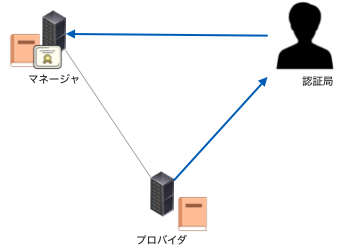
\includegraphics[scale=0.7]{figure/certificate-procedure.png}
 \caption{レコード情報操作におけるプロセスの概略図}
 \label{fig:manager-provider}
\end{figure}

DNS-TDでは,全てのコンテンツについて,信頼される第三者からストアしても良いと認可されていることを前提としている.
すなわち,ハッシュテーブル上のコンテンツへの操作,またはコンテンツをハッシュテーブル上にストアするなどの操作処理をする際,プロバイダは,信頼される第三者からのレコード情報に操作することを認可してもらう必要がある.
認可の証明書を発行する認証局は,プロバイダの基本情報とレコード情報に基づき証明書の発行を決定する.
いま,ドメイン名``www.example.com"のリソースレコードタイプAとして``93.184.216.34"というレコード情報を関連づけるとする.
プロバイダは,認証局に対して証明書発行リクエストを転送する.
認証局は,リクエストされたレコード情報についてIPアドレスの到達性と不審な文字列が含まれていないこと,利用目的について評価を施す.
認可された場合には,その証にディジタル証明書を発行し,マネージャにストアリクエストを転送する.
マネージャは,ディジタル証明書に付与された署名に基づきコンテンツの完全性を評価し,認証された場合コンテンツIDを計算し,担当マネージャにストアリクエストを転送する.
上記の手続きを経たコンテンツがハッシュテーブル上にストアされる.


\subsubsection{レコードタイプ}
本項では,DNS-TDで使用するリソースレコードのタイプについて説明する.

% 提案システムで使用するレコードタイプを概観するか,もしくは既存システムにおけるリソースレコードのタイプの課題から説明するのがいいだろう
はじめに,DNS-TDにおけるDNSSECの位置づけについて述べる.
DNSSEC~\cite{rfc4033}は,権威サーバからの応答パケットの偽装を検知することを目的として,データの作成元の確認とデータの完全性および,不在情報応答情報の証明するDNSの拡張仕様である.
これは,主としてDNSの応答パケットを偽装できる程度のパラメータであることに起因する.
他方で,DNS-TDでは,応答パケットに224bitのメッセージダイジェストが含まれるため,悪意のある応答パケットをフルサービスリゾルバに意図的にキャッシュすることは極めて困難である.以上の理由から,DNS-TDではDNSSECの目的にそぐわないため,リソースレコードとして使用されない.

次に,DNSSEC以外のリソースレコードについて説明する.
第~\ref{sec:dns-infiltration}項で示すように,既存の名前解決システムでドメインに関連づけることができるリソースレコードのいくつかのタイプは,DNS Infiltrationとして機能することができる.
DNS Infiltrationを抑止するリソースレコードであることの必要条件は,ドメインに関連のない任意の文字列がレコード情報に含められないことである.
既存のDNSのリソースレコードのタイプのうち,任意の文字列を含めることができるのタイプは以下の通りである.


表~\href{tab:infil-rtype}のDNS Infiltrationとして機能する可能性のあるリソースレコードのタイプのうち,IPアドレスを偽装して情報を転送するものについては,第~\ref{sec:certificate}項で述べた認証基盤によってレコード情報の正当性評価でスクリーニングすることができる.
他方で,任意の文字列を注入できるのが,NULL・TXT・CNAMEタイプである.

NULLについて考える.
NULLタイプの目的は,実験用と定義されている~\cite{rfc1035}.
TXTについて考える.
CNAMEについて考える.
ホスト名に対する別名で関連づけることができるCNAMEは,一つのサーバにおいてサービスごとにサーバの名前を変更させるために使用される.
%DNS-TDでは,ドメインごとにゾーンは保持しないので

% データベースについて
% Redisについて説明

%\subsection{データベース}
\subsubsection{コンテンツのデータフォーマット}
本項では,マネージャにて管理されるコンテンツのフォーマットについて説明する.

\begin{figure}[h]
 \centering
 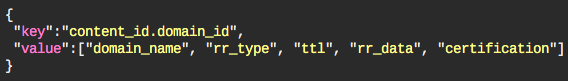
\includegraphics[scale=0.6]{figure/content-file.png}
 \caption{コンテンツのデータフォーマット}
 \label{fig:manager-provider}
\end{figure}

%\subsection{動作メカニズム}
%\subsubsection{レコード情報に対する操作}
%本項では,DNS-TDにおいて使用されるリソースレコードのタイプと
%%TTLの更新方法について説明する
%
%\subsubsection{名前解決}
%ハッシュテーブルのレプリケーション手法
%特定のハッシュ範囲を管理するノードは,複数用意させ,そのアドレスを対応表に明記し,ストアする際にその全てのレプリケーションサーバにストアリクエストする
